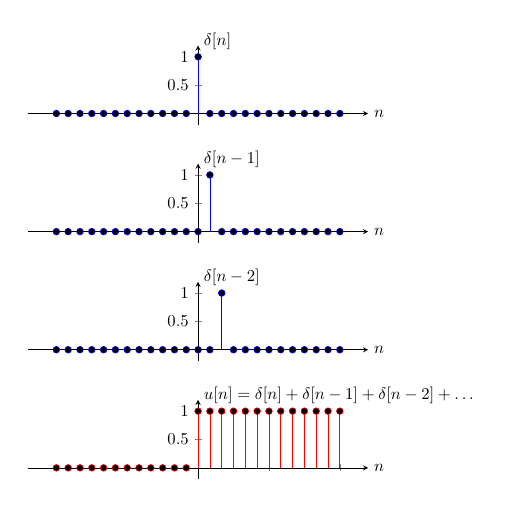
\begin{tikzpicture}[scale=0.6,
    declare function={
    unitstep(\x)= (\x>-0.1)*(1);
    impulse(\x,\nn)  = and((\nn-0.5) < \x, \x < \nn)*1;
  }
]
\begin{axis}
	[
	    scale=1,
	    axis x line=middle,
	    axis y line=middle,
	    every axis plot post/.style={mark options={fill=black}},
	    xmin=-12,
	    xmax=12,
	    xlabel={$n$},
	    ylabel={$\delta[n]$},
	    xticklabel=\empty,
	    y=1.2cm,
	    x=0.3cm,
	    ymin=-0.2,
	    ymax=1.2,
	    clip=false,
	     every axis x label/.style={at={(ticklabel* cs:1)}, anchor=west,} ,
	     every axis y label/.style={at={(ticklabel* cs:1.05)}, anchor=west,},
	]
	\addplot+[ycomb,domain=-10:10, blue] {impulse(x,0)};
\end{axis}

\pause

\begin{scope}[yshift=-2.5cm]
	\begin{axis}
	[
	    scale=1,
	    axis x line=middle,
	    axis y line=middle,
	    every axis plot post/.style={mark options={fill=black}},
	    xmin=-12,
	    xmax=12,
	    xlabel={$n$},
	    ylabel={$\delta[n-1]$},
	    xticklabel=\empty,
	    y=1.2cm,
	    x=0.3cm,
	    ymin=-0.2,
	    ymax=1.2,
	    clip=false,
	     every axis x label/.style={at={(ticklabel* cs:1)}, anchor=west,} ,
	     every axis y label/.style={at={(ticklabel* cs:1.05)}, anchor=west,},
	]
	\addplot+[ycomb,domain=-10:10, blue] {impulse(x,1)};
	\end{axis}
\end{scope}

\pause

\begin{scope}[yshift=-5cm]
	\begin{axis}
	[
	    scale=1,
	    axis x line=middle,
	    axis y line=middle,
	    every axis plot post/.style={mark options={fill=black}},
	    xmin=-12,
	    xmax=12,
	    xlabel={$n$},
	    ylabel={$\delta[n-2]$},
	    xticklabel=\empty,
	    y=1.2cm,
	    x=0.3cm,
	    ymin=-0.2,
	    ymax=1.2,
	    clip=false,
	     every axis x label/.style={at={(ticklabel* cs:1)}, anchor=west,} ,
	     every axis y label/.style={at={(ticklabel* cs:1.05)}, anchor=west,},
	]
	\addplot+[ycomb,domain=-10:10, blue] {impulse(x, 2)};
	\end{axis}
\end{scope}


\pause

\begin{scope}[yshift=-7.5cm]
	\begin{axis}
	[
	    scale=1,
	    axis x line=middle,
	    axis y line=middle,
	    every axis plot post/.style={mark options={fill=black}},
	    xmin=-12,
	    xmax=12,
	    xlabel={$n$},
	    ylabel={$u[n] = \delta[n] + \delta[n-1] + \delta[n-2] + \dots$},
	    xticklabel=\empty,
	    y=1.2cm,
	    x=0.3cm,
	    ymin=-0.2,
	    ymax=1.2,
	    clip=false,
	     every axis x label/.style={at={(ticklabel* cs:1)}, anchor=west,} ,
	     every axis y label/.style={at={(ticklabel* cs:1.05)}, anchor=west,},
	]
	\addplot+[ycomb,domain=-10:10, red] {unitstep(x)};
	\end{axis}
\end{scope}
\end{tikzpicture} 